\documentclass[a4paper,11pt]{article}

% ---------- Fonts and page layout (Tectonic / XeTeX; see docs/explain_docs precedent) ----------
\usepackage{fontspec}
\setmainfont{TeX Gyre Termes}
\setsansfont{TeX Gyre Heros}
\setmonofont{DejaVu Sans Mono}

\usepackage[a4paper,left=25mm,right=25mm,top=25mm,bottom=25mm]{geometry}
\usepackage{setspace}
\setstretch{1.10}

\usepackage{amsmath,amssymb}
\usepackage{graphicx}
\usepackage{booktabs}
\usepackage{tabularx}
\usepackage{multirow}
\usepackage{makecell}
\usepackage{caption}
\captionsetup{font=small,labelfont=bf}
\usepackage[hidelinks]{hyperref}
\usepackage{natbib}
\bibliographystyle{plainnat}

% AUTO-GENERATED by scripts/build_wp_tables_v11.py -- do not edit by hand.
\newcommand{\LoneNasof}{3}
\newcommand{\LoneCells}{15}
\newcommand{\LoneNegative}{15}
\newcommand{\LoneBestExcess}{-8.2}
\newcommand{\LoneWorstExcess}{-59.7}
\newcommand{\LoneSpecTotal}{27}
\newcommand{\LoneEnd}{2026-06-01}
\newcommand{\PanelFilings}{10{,}712}
\newcommand{\PanelFirms}{3{,}579}
\newcommand{\PanelYears}{3}
\newcommand{\LoneADate}{2024-10-01}
\newcommand{\LoneAGate}{87}
\newcommand{\LoneAScreenable}{2{,}224}
\newcommand{\LoneAPoolT}{-2.36}
\newcommand{\LoneAMonths}{19}
\newcommand{\LoneATopix}{29.4}
\newcommand{\LoneAPoolAnn}{6.7}
\newcommand{\LoneAPoolExcess}{-22.8}
\newcommand{\LoneAPoolBeta}{0.71}
\newcommand{\LoneATopFiveAnn}{4.5}
\newcommand{\LoneATopTwentyAnn}{15.5}
\newcommand{\LoneBDate}{2025-04-01}
\newcommand{\LoneBGate}{153}
\newcommand{\LoneBScreenable}{3{,}111}
\newcommand{\LoneBPoolT}{-1.94}
\newcommand{\LoneBMonths}{14}
\newcommand{\LoneBTopix}{41.8}
\newcommand{\LoneBPoolAnn}{14.5}
\newcommand{\LoneBPoolExcess}{-27.2}
\newcommand{\LoneBPoolBeta}{0.74}
\newcommand{\LoneBTopFiveAnn}{-14.2}
\newcommand{\LoneBTopTwentyAnn}{32.1}
\newcommand{\LoneCDate}{2025-10-01}
\newcommand{\LoneCGate}{176}
\newcommand{\LoneCScreenable}{3{,}377}
\newcommand{\LoneCPoolT}{-3.15}
\newcommand{\LoneCMonths}{8}
\newcommand{\LoneCTopix}{46.0}
\newcommand{\LoneCPoolAnn}{-3.3}
\newcommand{\LoneCPoolExcess}{-49.3}
\newcommand{\LoneCPoolBeta}{0.74}
\newcommand{\LoneCTopFiveAnn}{-13.6}
\newcommand{\LoneCTopTwentyAnn}{12.9}
\newcommand{\LtwoSeed}{20260725}
\newcommand{\LtwoDraws}{10{,}000}
\newcommand{\LtwoPool}{1{,}469}
\newcommand{\LtwoActualHoldings}{20}
\newcommand{\LtwoInsidePool}{20}
\newcommand{\LtwoActualAnn}{53.8}
\newcommand{\LtwoActualBeta}{1.06}
\newcommand{\LtwoActualMdd}{-30.0}
\newcommand{\LtwoUnstratMedian}{23.2}
\newcommand{\LtwoMatchedMedian}{31.7}
\newcommand{\LtwoUnstratPctile}{100.0}
\newcommand{\LtwoMatchedPctile}{99.9}
\newcommand{\LtwoMatchedBetaPctile}{99.7}
\newcommand{\LtwoMatchedMddPctile}{1.6}
\newcommand{\LtwoMatchedBetaMedian}{0.89}
\newcommand{\FaMonths}{36}
\newcommand{\FaFirst}{2023-07}
\newcommand{\FaLast}{2026-06}
\newcommand{\FaSectorName}{Electric Appliances}
\newcommand{\FaQmjAnn}{-0.1}
\newcommand{\FaSizeAnn}{-11.3}
\newcommand{\FaSectorAnn}{+12.4}
\newcommand{\FaMomAnn}{+10.3}
\newcommand{\FaOursAlpha}{+17.8}
\newcommand{\FaHeadOursAlpha}{+12.7}
\newcommand{\FaHeadOursAlphaT}{+2.09}
\newcommand{\FaHeadOursSector}{0.82}
\newcommand{\FaHeadOursSectorT}{+2.82}
\newcommand{\FaHeadOursRtwo}{0.72}
\newcommand{\FaHeadBenchAlpha}{+14.6}
\newcommand{\FaHeadBenchAlphaT}{+1.90}
\newcommand{\FaGrahamAnn}{13.3}
\newcommand{\FaGrahamTopix}{24.0}
\newcommand{\FaOursAlphaT}{+2.29}
\newcommand{\FaOursSector}{0.98}
\newcommand{\FaOursSectorT}{+3.44}
\newcommand{\FaOursCapmAlpha}{+12.6}
\newcommand{\FaBenchAlpha}{+23.9}
\newcommand{\FaBenchAlphaT}{+3.06}
\newcommand{\FaOursRtwo}{0.75}
\newcommand{\DofMin}{29.1}
\newcommand{\DofMax}{80.6}
\newcommand{\DofSpread}{51.5}
\newcommand{\DofVariants}{9}
\newcommand{\SpecTotal}{85}
\newcommand{\SpecBreakdown}{27 layer 1 as-of validation; 4 layer 2 randomisation; 12 factor attribution; 9 benchmark construction (contribution B); 8 quality-gate threshold robustness (contest edition); 4 market-phase splits (contest edition); 3 allocation rules (contest edition); 2 measurement windows (contest edition); 4 benchmark comparison pairs (contest edition); 1 volatility-matched leverage variant (contest edition); 1 graham-style control (contest edition); 10 cost conventions (this paper)}
\newcommand{\CostOneWay}{25}
\newcommand{\CostOddLot}{15}
\newcommand{\CostTurnover}{1.07}
\newcommand{\CostHeadlineAnn}{52.8}
\newcommand{\CostContestAnn}{53.8}
\newcommand{\CostDrag}{1.0}
\newcommand{\CostGridMax}{100}
\newcommand{\CostHundredBp}{51.2}
\newcommand{\DsrObserved}{1.79}
\newcommand{\DsrThreshold}{0.63}
\newcommand{\DsrProb}{0.972}
\newcommand{\DsrKurtosis}{11.70}
\newcommand{\SatFirms}{3{,}649}
\newcommand{\SatDistinct}{20}
\newcommand{\SatEffLevels}{3.91}
\newcommand{\SatTopFiveShare}{90.2}
\newcommand{\SatSectorShare}{99.0}
\newcommand{\SatSingleSectors}{18}
\newcommand{\SatSectors}{33}
\newcommand{\SatTieN}{273}
\newcommand{\SatTieValue}{0.9723}
\newcommand{\SatAbove}{3}
\newcommand{\SatRdPresent}{2}
\newcommand{\SatShareCount}{300}
\newcommand{\SatRdImputed}{3{,}647}
\newcommand{\LadderPool}{1{,}200}
\newcommand{\LadderLzero}{600}
\newcommand{\LadderLone}{586}
\newcommand{\LadderLtwo}{8}
\newcommand{\LadderLthree}{6}
\newcommand{\LadderVerified}{14}
\newcommand{\LadderKeywordOnly}{577}
\newcommand{\OwnHoldings}{20}
\newcommand{\OwnPresent}{15}
\newcommand{\OwnAbsent}{5}
\newcommand{\OwnLevelZero}{5}
\newcommand{\OwnLevelOne}{9}
\newcommand{\OwnLevelTwo}{1}
\newcommand{\OwnVerified}{1}
\newcommand{\OwnOverlap}{1}
\newcommand{\SurvTickers}{3{,}650}
\newcommand{\SurvStart}{2021-06-01}
\newcommand{\SurvEnd}{2026-06-01}
\newcommand{\SurvStopped}{1}
\newcommand{\SurvThreshold}{30}
\newcommand{\MdeA}{+24.3}
\newcommand{\MdeATe}{11.0}
\newcommand{\MdeADetect}{below the detection threshold}
\newcommand{\MdeB}{+32.2}
\newcommand{\MdeBTe}{12.2}
\newcommand{\MdeBDetect}{below the detection threshold}
\newcommand{\MdeC}{+36.5}
\newcommand{\MdeCTe}{10.4}
\newcommand{\MdeCDetect}{detectable}
\newcommand{\MdeNotDetectable}{2}
\newcommand{\LoneRejectFive}{2}
\newcommand{\MdeTotal}{3}


\title{\textbf{When Keyword Measures of Thematic Exposure Break Down:\\
Can a Disclosure-Based Evidence Ladder Substitute?}\\[2mm]
\large An identification-explicit case study in Japanese equities}
\author{[Author names withheld in this draft]\\\small Undergraduate research team}
\date{Draft of \today\ --- \emph{working paper circulated for comment}}

\begin{document}
\maketitle

\begin{abstract}
\noindent Measures of a firm's exposure to an investment theme are commonly built by matching keywords
against firm text. We audit one such measure across \SatFirms\ Japanese listed firms and find that it
\emph{saturates}: it takes \SatDistinct\ distinct values, and \SatSectorShare\% of firms sit exactly at
their own sector's median. \SatTieN\ firms --- a semiconductor photomask-inspection monopolist, a
fire-alarm maker, a watchmaker, a railway-signalling firm --- carry an identical score. The mechanism
is checkable: the keyword match reads firm metadata rather than disclosure text, a sector bonus is
hard-coded on top, and the one continuous firm-level input is populated for \SatRdPresent\ of
\SatFirms\ firms. Arithmetically the measure is a sector label. We propose a disclosure-graded
\emph{evidence ladder} as the alternative and define it as a coding protocol, then turn it on the
portfolio this paper studies: of \OwnHoldings\ holdings, \OwnVerified\ carries artefact-backed thematic
evidence. We believed our own selection was evidence-based; it was not, and we could not tell from the
inside. Performance claims are partitioned into three layers and calibrated within them: out-of-sample,
the mechanical screen shows no evidence of adding value (\LoneNegative\ of \LoneCells\ specification
cells underperform TOPIX) under a design too weak to license the stronger negative claim; the full
portfolio sits high in a randomisation distribution and equally high in that distribution's beta and
drawdown tails; and its factor alpha, while surviving a sector control, is \emph{smaller} than the
alpha of the purely mechanical benchmark built from the same gate. The contribution is a measurement
one. Every number is generated by scripts in the replication package, and the \SpecTotal\ specifications
we traversed are counted and disclosed.
\end{abstract}

\medskip
\noindent\fbox{\begin{minipage}{0.97\textwidth}\small
\textbf{What this paper does not claim.} It does not claim that the portfolio studied here beat any
benchmark out-of-sample; Table~\ref{tab:layer1} says the opposite for the part we can test. It does
not claim the evidence ladder predicts returns --- we have not validated it against realised
fundamentals, and we say what such a validation would require. Comparisons to a
Buffett-style benchmark appear only as the motivating story that produced the data, and are
reported inside the layer that owns them.
\end{minipage}}

\section{Motivation}\label{sec:motivation}

This paper began as an undergraduate stock-selection project and became a measurement paper by
accident. We were building a portfolio around exposure to the AI investment theme, and we needed to
rank Japanese firms by how exposed they were. We had a composite AI-exposure score of the ordinary
kind, so we sorted on it.

The sort did not work. One of our candidate holdings, santec, makes tunable lasers and optical test
instruments --- a plausible beneficiary of optical interconnect demand in data centres. Its score was
\SatTieValue. So was the score of \SatTieN\ other firms, among them Lasertec, the sole global supplier
of photomask inspection systems for EUV lithography, and also a fire-alarm manufacturer, a watch
company, and a railway signalling firm. Only \SatAbove\ firms in the entire market scored higher than
any of them. We could not use the measure to choose between a monopolist in advanced semiconductor
metrology and a maker of smoke detectors, because the measure did not distinguish them.

Our first reaction was that we had found a quirk in one index. Investigating the construction
(Section~\ref{sec:saturation}) showed something more systematic, and turning our own proposed
remedy back on our own portfolio (Section~\ref{sec:own-audit}) showed that we had been relying on the
broken measure without knowing it. That sequence --- a measure that cannot rank, a mechanism that
explains why, and a study that failed its own test --- is what the paper reports. The portfolio's
performance appears here only as the vehicle that carried us to the question, reported inside the
identification layer that owns it.

\section{The measurement problem}\label{sec:measurement}

\subsection{Saturation, and the mechanism behind it}\label{sec:saturation}

We audit the thematic-exposure score that our own selection pipeline inherited --- a composite
AI-exposure index of exactly the kind an investor would take off the shelf --- across all
\SatFirms\ firms in the cross-section. Table~\ref{tab:saturation} reports what it resolves.

The score takes \SatDistinct\ distinct values. Its five largest ties account for
\SatTopFiveShare\% of all firms, and the effective number of levels, computed as the inverse
Herfindahl index of the tie-size shares, is \SatEffLevels. \SatTieN\ firms share the single value
\SatTieValue, and only \SatAbove\ firms in the entire market score above them. Inside that tie sit
Lasertec, the sole global supplier of photomask inspection systems for advanced semiconductor
lithography, and --- indistinguishably --- a fire-alarm manufacturer, a watchmaker, and a railway
signalling company. This is not noise around a usable signal. In the region of the distribution where
an investor needs the measure to discriminate, it does not order firms at all.

The mechanism is worth stating precisely, because it is specific and checkable rather than a general
complaint about keyword methods. Three construction choices compound:

\begin{enumerate}\itemsep2pt
\item \textbf{The keyword match never reads a disclosure.} It runs over firm metadata --- company
name, the 33- and 17-sector labels, market segment, and scale category. A firm can reach a theme
bucket without ever having mentioned the theme, and a firm that discusses it at length in its filings
gains nothing.
\item \textbf{A hard-coded sector bonus is added.} Membership in Electric Appliances, Machinery,
Chemicals, Nonferrous Metals, Metal Products, or Precision Instruments adds a fixed increment to the
AI-infrastructure bucket, with parallel bonuses for the other buckets. Since the sector label is also
one of the matched text fields, sector enters twice.
\item \textbf{The only continuous firm-level input is missing and silently imputed.} R\&D intensity
carries a quarter of the composite's weight. It is populated for \SatRdPresent\ of
\SatFirms\ firms and filled with zero for the remaining \SatRdImputed.
\end{enumerate}

Together these leave nothing that varies across firms within a sector. The arithmetic consequence is
visible in the data: \SatSectorShare\% of firms sit exactly at their sector's median score, and
\SatSingleSectors\ of \SatSectors\ sectors are single-valued --- every firm in them receives an
identical score. \textbf{The measure is a sector label presented as a firm-level exposure
estimate.} We emphasise that we found this by auditing a measure we had ourselves relied on, and that
the failure is not exotic: each of the three choices above is individually defensible, and a user who
never inspects the missingness of one input would not see the result.

We take the general lesson to be about the direction of the field's remedy rather than about this one
index. \citet{HobergPhillips2016} construct industry classifications from firm-written product
descriptions precisely because assigned sector codes lose firm-specific information; a thematic
measure that reduces to a sector code has thrown away the same information while appearing not to.
The diagnostic is cheap and, we would argue, should be routine: report the number of distinct values a
proposed exposure measure takes, and the share of firms sitting at their sector's median.

% AUTO-GENERATED by scripts/build_wp_tables_v11.py -- do not edit by hand.
\begin{table}[htbp]
\centering\small
\caption{\textbf{Measurement audit (no inference layer).} \emph{Saturation of a thematic-exposure measure.} This table makes no claim about returns. All 3{,}649 listed firms in the cross-section, scored by the composite AI-exposure index inherited by our own pipeline.}
\label{tab:saturation}
\begin{tabular}{lr}
\toprule
\multicolumn{2}{l}{\textit{Resolution}} \\
Firms scored & 3{,}649 \\
Distinct score values & 20 \\
Effective number of levels (inverse Herfindahl) & 3.91 \\
Five largest ties, share of cross-section & 90.2\% \\
Firms exactly at their sector's median score & 99.0\% \\
Single-valued sectors & 18 of 33 \\
\midrule
\multicolumn{2}{l}{\textit{The largest tie at the top: 273 firms at a score of 0.9723, with 3 firms above}} \\
\quad Lasertec Corporation \textit{(semiconductor photomask inspection; sole global supplier)} & --- \\
\quad HOCHIKI CORPORATION \textit{(fire alarms and detection equipment)} & --- \\
\quad Citizen Watch Co.,Ltd. \textit{(wristwatches)} & --- \\
\quad Nippon Signal Company,Limited \textit{(railway signalling)} & --- \\
\quad santec Holdings Corporation \textit{(optical test instruments for fibre networks)} & --- \\
\midrule
\multicolumn{2}{l}{\textit{Mechanism}} \\
Keyword match reads disclosure text? & \textbf{No} \\
Fields matched & metadata only\rlap{$^{a}$} \\
R\&D intensity (weight 0.25) populated for & 2 of 3{,}649 firms \\
\bottomrule
\end{tabular}
\begin{minipage}{\textwidth}\vspace{2pt}\scriptsize
$^{a}$ Company name, 33-sector label, 17-sector label, market segment, scale category; plus a hard-coded additive bonus for membership in designated sectors. Since the sector label is both a matched field and a bonus trigger, sector enters twice, and no remaining input varies across firms within a sector.
\end{minipage}
\end{table}

\begin{table}[htbp]
\centering\small
\caption{\textbf{Measurement audit (no inference layer).} \emph{The evidence ladder, and what our own portfolio scores on it.} Top-1200 candidate pool from the contest edition's value-quality screen. Levels 0 and 1 are assigned by script; levels 2 and 3 each carry a source URL, source type, and quoted passage.}
\label{tab:ladder}
\begin{tabular}{llrr}
\toprule
Level & Requirement & Firms & Share \\
\midrule
\multicolumn{4}{l}{\textit{Panel A: the candidate pool}} \\
0 & No thematic keyword link & 600 & 50.0\% \\
1 & Keyword hit only; no artefact & 586 & 48.8\% \\
2 & Named product, customer, or committed investment & 8 & 0.7\% \\
3 & Disclosed quantity attributable to the theme & 6 & 0.5\% \\
\midrule
\multicolumn{2}{l}{Verified by hand (levels 2--3)} & 14 & 1.2\% \\
\multicolumn{2}{l}{Discarded as keyword-only} & 577 & \\
\midrule
\multicolumn{4}{l}{\textit{Panel B: the same ladder applied to the 20 holdings this paper studies}} \\
0 & No thematic keyword link & 5 & 25.0\% \\
1 & Keyword hit only & 9 & 45.0\% \\
2 & Named product or customer & 1 & 5.0\% \\
3 & Disclosed quantity & 0 & 0.0\% \\
--- & \emph{Never scored (outside the pool)} & 5 & 25.0\% \\
\bottomrule
\end{tabular}
\begin{minipage}{\textwidth}\vspace{2pt}\scriptsize
\textit{Notes.} The ladder's discriminating power is concentrated in the 14 firms where a human opened a document. The 577 discarded firms' filings were \emph{not} read; they are the residual after hand verification, not a population that was inspected and rejected. The ladder is \textbf{not validated} as a predictor --- see Section~\ref{sec:ladder-validation} for what a validation would require.
\end{minipage}
\end{table}



\subsection{An evidence ladder, defined so it can be re-coded}\label{sec:ladder}

If keyword presence cannot order firms, the alternative is to grade what a firm's disclosures actually
substantiate. We define three levels, stated as a coding protocol rather than a concept, and report
their distribution over the \LadderPool-firm candidate pool in Table~\ref{tab:ladder}.

\textbf{Level 1 --- keyword only.} A keyword places the firm in a theme bucket, and no retrievable
artefact names a product, a customer, or a committed investment. Assigned mechanically.

\textbf{Level 2 --- named product or customer.} A retrievable artefact (a filing passage, product
page, or IR document) names a specific product, customer, or committed investment tied to the theme.
The coder records the source URL, the source type, and the quoted passage.

\textbf{Level 3 --- disclosed quantity.} The artefact carries a number attributable to the theme:
revenue, order book, unit or customer count, or capital expenditure, with its as-of date. The number
and the quotation are both recorded.

The distribution is the point. Of \LadderPool\ firms, \LadderLzero\ have no thematic link at all and
\LadderLone\ are level 1 --- keyword-reachable and nothing more. Only \LadderLtwo\ reach level 2 and
\LadderLthree\ reach level 3. The ladder's discriminating power is concentrated in the
\LadderVerified\ firms where a human opened a document; everything else is the saturated region of
Section~\ref{sec:saturation} under a different name. Every level-2 and level-3 assignment in this
study carries a URL and a quoted snippet, so a referee can re-open the artefact and disagree with the
coding. Levels 0 and 1 require no judgement and are reproducible by script.

\paragraph{What the \LadderKeywordOnly\ figure does and does not mean.} Our own earlier write-up reported that \LadderKeywordOnly\ 
firms were excluded as ``keyword-only''. Stated carelessly this sounds like \LadderKeywordOnly\ sets of filings read
and found wanting. It is the opposite: it is the residual after \LadderVerified\ firms were verified
by hand, discarded as a block. \textbf{Those \LadderKeywordOnly\ firms' filings were not read.} We correct the
phrasing here because the looser version credits the study with work it did not do.

\subsection{Applying the ladder to our own portfolio}\label{sec:own-audit}

The obvious test of a proposed measure is to turn it on the study that proposes it. We did that late,
and it produced the most uncomfortable result in this paper.

Of the \OwnHoldings\ holdings in the portfolio whose performance we report,
\OwnAbsent\ never entered the candidate pool and so were never assigned a thematic level at all.
Among the \OwnPresent\ that were, \OwnLevelTwo\ carries a hand-verified level-2 artefact ---
Lasertec, with a quoted statement about EUV mask-blank inspection and a source URL.
\OwnLevelOne\ sit at level 1: reachable by the metadata keyword screen and nothing more.
\OwnLevelZero\ sit at level 0, with no thematic keyword link at all. And the portfolio shares only
\OwnOverlap\ name with the selection pipeline's own final-20 list.

\textbf{The thematic leg of our own portfolio does not clear the ladder we are proposing.} It sits
almost entirely inside the saturated region of Section~\ref{sec:saturation} --- the region we argue is
uninformative. The working file that records the role rationales states, at the top, that the business
descriptions are drafted from general knowledge and require verification against IR and EDINET before
submission; for these fifteen holdings that verification was never completed. We had described the
selection in an earlier draft as reading disclosures. It was not.

We report this for three reasons. It is true. It changes what Layer 2 can mean: the randomisation
result in Section~\ref{sec:layer2} compares a discretionary portfolio against random draws, but the
discretion was narrative rather than evidentiary, so ``selection skill'' is not even the right name
for what is being tested. And it relocates this paper's motivation honestly. The evidence ladder is
not proposed because other people's measures are poor. It is proposed because our own selection
process, which we believed was evidence-based, turns out on inspection to have been keyword-and-story
based for nineteen of twenty holdings --- and we could not tell from the inside. That is the failure
mode we think is general, and it is the reason the diagnostic in Section~\ref{sec:saturation} should
be routine rather than exceptional.

\paragraph{We have not validated the ladder.}\label{sec:ladder-validation} Nothing above shows the
ladder predicts anything. It is a measurement proposal with a coding protocol, not a tested signal,
and the honest description of its status is that it survived only the test of being cheaper to
disagree with than a keyword count. A validation would need, at minimum: coding the ladder at an
as-of date from filings available at that date, on a sample large enough for a cross-sectional test;
a pre-specified outcome, for which realised theme-attributable revenue growth is the natural choice
and is disclosed by only a minority of firms; inter-coder agreement statistics, since levels 2 and 3
require judgement that \LadderVerified\ hand assignments cannot establish; and a head-to-head
comparison against the saturated measure on the same sample and horizon.

The crudest possible version of that test is in Appendix Table~\ref{tab:correspondence}, and it does
not favour us: among the \LadderVerified\ hand-coded firms, those at level 3 grew revenue
\emph{more slowly} over the window than those at level 2. We report it because a paper arguing for
careful measurement cannot omit the one descriptive check it can compute merely because the check is
unflattering --- but we would resist any reading of it, in either direction, for the reasons given in
the table's notes. Designing the study that could actually order the levels is the question we would
most like a reader's view on, and it is the second question in our cover letter.

\section{Data and identification}\label{sec:data}

\subsection{The point-in-time panel}

Our accounting data is a panel of annual securities reports filed with EDINET: \PanelFilings\ filings
covering \PanelFirms\ firms, a median of \PanelYears\ fiscal years each. Each filing carries its \emph{submission timestamp}
alongside the fiscal period it covers, and that single field is what makes Layer 1 possible. It lets
us reconstruct, for any date, exactly which firms' financials a screen could have seen --- a
distinction that a panel indexed only by fiscal period silently erases, because a fiscal year ending
in March is not public until it is filed, typically three months later. The funnel in Appendix
Table~\ref{tab:layer1-t} reports how much of the cross-section is visible at each of our as-of dates:
at \LoneADate, \LoneAGate\ firms clear the quality gate out of the \LoneAScreenable\ firms with enough filing
history to screen, and most of the attrition is firms with only one fiscal year on file rather than
firms failing the gate.

Prices are daily adjusted closes for \SurvTickers\ tickers from \SurvStart\ to \SurvEnd. We adjust
the TOPIX ETF (1306.T) for its ten-for-one split on 2026-03-30; unadjusted, that split alone would
misstate every benchmark return in this paper by an order of magnitude, and we flag it because it is
the kind of error that survives peer review. The panel contains essentially only tickers still
listed at the end date --- exactly \SurvStopped\ series stops more than thirty days early --- so it is
a survivors-only panel. Section~\ref{sec:limitations} states the direction of the resulting bias and
declines to estimate its size.

Two variables we do \emph{not} have shape the whole design. There are no point-in-time share counts,
and the 2026 snapshot of shares outstanding covers \SatShareCount\ of \SatFirms\ firms, chosen by the
2026 scoring pipeline. This is why the Layer 1 ranking drops the valuation leg
(Section~\ref{sec:l1scope}) and why the factor model has no value factor
(Section~\ref{sec:factors}). And we have no delisting list, which is why survivorship is a stated
direction rather than a number.

\subsection{Three layers of claims}\label{sec:layers}

Every empirical claim in this paper belongs to exactly one of the three layers in
Table~\ref{tab:layers}, and each results table is labelled with its layer. The purpose of the
partition is to stop a strong in-sample number from borrowing credibility from a weak
out-of-sample design, or the reverse.

\begin{table}[htbp]
\centering\small
\caption{\textbf{The three-layer separation of claims.} Declared before the analyses were run.}
\label{tab:layers}
\renewcommand{\arraystretch}{1.25}
\begin{tabularx}{\textwidth}{@{}l>{\raggedright\arraybackslash}X>{\raggedright\arraybackslash}X>{\raggedright\arraybackslash}X@{}}
\toprule
& \textbf{L1 --- Out-of-sample} & \textbf{L2 --- Randomisation} & \textbf{L3 --- Description} \\
\midrule
\emph{Object} &
The part of the selection fixed by a mechanical formula &
The final 20-firm portfolio, including its discretionary holdings &
Behaviour by market phase and by assigned role \\
\emph{Information set} &
Only filings on file at each as-of date &
2026 information; hindsight is present by construction &
Same as L2 \\
\emph{Inference allowed} &
Conventional tests, with power limits stated first &
Percentile against a placebo distribution only &
Descriptive statistics only \\
\emph{Not permitted} &
Any suggestion that the discretionary 15 firms were reproduced &
$t$-statistics; the word ``significant'' &
Any inferential vocabulary \\
\bottomrule
\end{tabularx}
\begin{minipage}{\textwidth}\vspace{2pt}\scriptsize
\textit{Notes.} Two further table labels appear, and we define them here rather than leave a reader to
infer the rule. \emph{Measurement audit} (Section~\ref{sec:measurement}) reports properties of a
measure rather than of a portfolio and makes no claim about returns. \emph{Attribution}
(Sections~\ref{sec:factors} and~\ref{sec:costs}) reports regression and Sharpe statistics for a
portfolio formed with 2026 information; those statistics measure \emph{how much of an already-known
in-sample return tradable factor exposures span}, and are not inference about future performance or
about skill. This is why the attribution tables carry $t$-statistics while Layers 2 and 3 do not: the
prohibition in the last row applies to inference about the portfolio's merit, and an attribution
regression makes no such claim. We flag the tension rather than resolve it by relabelling, and it is
part of what our third question to readers asks about. Every table in this paper carries one of these
five labels.
\end{minipage}
\end{table}

\subsection{What Layer 1 can and cannot reproduce}\label{sec:l1scope}

The portfolio studied here was assembled in three groups of five firms plus two smaller groups. Only
the first group is fixed by a formula. \textbf{The remaining fifteen holdings rest on discretionary
judgement that cannot be reproduced point-in-time}: the judgement was exercised in 2026 and is not
recoverable from any archived variable, so no as-of reconstruction of it would be honest. Layer 1
therefore validates the quality gate and the quality ranking --- not the portfolio.

We must be precise about what that discretion consisted of, because an earlier draft of this paper
described it as reading company disclosures, and our own records do not support that description.
Section~\ref{sec:own-audit} reports the audit. The accurate statement is that the fifteen holdings
rest on narrative judgement informed by general familiarity with the firms, and that exactly
\OwnVerified\ holding carries artefact-backed thematic evidence.

The mechanical part is at least stable: perturbing any single threshold in the gate leaves at least
four of the five holdings in place (Appendix Table~\ref{tab:robustness}). That is a property of the
rule on one snapshot, not evidence about returns, and we flag it here only so a reader does not
mistake the Layer 1 null for knife-edge sensitivity to a threshold.

Two further deviations are forced by the data and are disclosed here rather than in a footnote.
First, the contest screen requires three consecutive loss-free fiscal years; at the earliest as-of
date only two years are on file for most firms, so the gate is \emph{translated} to ``loss-free over
the periods available at the as-of date,'' and the number of available periods is reported for each
as-of date. Second, the contest ranking adds an earnings-yield rank to an ROE rank, and an earnings
yield needs a share count; no point-in-time share counts exist in our data, and the 2026 snapshot
covers only \SatShareCount\ of \SatFirms\ firms --- a set chosen by the 2026 scoring pipeline,
so screening on it
would inject selection look-ahead into the as-of pool. The Layer 1 ranking is consequently the
quality leg alone, with an ROE-plus-margin rank sum reported alongside it.

\subsection{Statistical power, stated before the results}\label{sec:power}

We state what this design can detect before showing what it found, because the answer bounds every
interpretation in Section~\ref{sec:results} --- including the interpretation that favours us least,
and the one that favours us most.

Layer 1 has \LoneNasof\ as-of dates with forward windows of \LoneAMonths, \LoneBMonths, and
\LoneCMonths\ months, and the pools overlap heavily, so this is not three independent
observations. Taking the realised tracking error of the equal-weighted pool against TOPIX at each
as-of date --- \MdeATe\%, \MdeBTe\%, and \MdeCTe\% annualised --- the minimum excess return
detectable two-sided at the 5\% level with 80\% power is \MdeA, \MdeB, and \MdeC\ percentage points
respectively. These thresholds are enormous, and they have a consequence we want stated in advance:
at \MdeNotDetectable\ of the \MdeTotal\ as-of dates, the shortfall we go on to observe is
\emph{smaller in magnitude than what the test could reliably detect}.

A caution about how to combine this with the test statistics we report, because the two are easy to
conflate and point in different directions. The minimum detectable effect is computed at 80\% power,
which is a stricter bar than significance at the 5\% level: it asks what effect size the design would
reliably find, not what it would occasionally flag. Consequently an estimate can clear the
significance threshold while sitting below the detection threshold, and in our results
\LoneRejectFive\ of the \MdeTotal\ as-of dates do exactly that --- the equal-weighted pool's excess
return is distinguishable from zero at the 5\% level (Newey--West $t$ of \LoneAPoolT\ and
\LoneCPoolT; see Appendix Table~\ref{tab:layer1-t}) while lying inside the 80\%-power interval.

The correct reading of that combination is not that the estimates are noise --- our own $t$-statistics
reject --- and not that the gate is shown to destroy value. It is that \textbf{a design with this
little power that nonetheless rejects is telling us something fragile.} If an effect of the size we
observe were the truth, this design would miss it more often than one time in five; a rejection
produced under those conditions is as consistent with the regime the windows happen to cover as with
a property of the gate. We therefore decline the strong negative claim, and the defensible reading is
the narrow one: \textbf{there is no evidence here that the mechanical gate produced the portfolio's
in-sample return, and the design was never capable of establishing that it did.}

We count \SpecTotal\ distinct specifications traversed across this paper and the contest edition
that preceded it, enumerated by category in Section~\ref{sec:costs}, and we use that count to
deflate the Sharpe ratio \citep{BaileyLopezdePrado2014} rather than reporting a raw one.

\section{Results}\label{sec:results}

\subsection{Layer 1: the mechanical screen out-of-sample}

Table~\ref{tab:layer1} re-forms the screen at each as-of date and measures forward to \LoneEnd.
The result is uniformly negative. At \LoneADate, \LoneAGate\ firms pass the translated gate; the
equal-weighted pool returns \LoneAPoolAnn\% annualised against \LoneATopix\% for TOPIX over the
following \LoneAMonths\ months (\LoneAPoolExcess\ percentage points), with a beta of
\LoneAPoolBeta. At \LoneBDate\ the pool excess is \LoneBPoolExcess\ points, and at \LoneCDate\ it is
\LoneCPoolExcess\ points. Concentrating the screen does not help: the mechanical top-five returns
\LoneATopFiveAnn\%, \LoneBTopFiveAnn\%, and \LoneCTopFiveAnn\% at the three dates respectively.
All \LoneCells\ cells underperform the benchmark.

Two readings are available and we cannot separate them with this design. The screen selects
low-beta, high-margin, high-equity-ratio firms, and the forward windows fall in a sharp market
advance in which such firms lagged --- every portfolio beta in Table~\ref{tab:layer1} is at or below
one. That is a regime explanation. Alternatively the gate has no forward-looking content in this
market. Distinguishing the two requires the factor attribution of Section~\ref{sec:factors}, and
even then \LoneNasof\ overlapping as-of dates cannot settle it.

Nor, as Section~\ref{sec:power} warned, can the table support the stronger negative claim. At
\LoneADate\ and \LoneBDate\ the observed shortfalls of \LoneAPoolExcess\ and \LoneBPoolExcess\ points
sit inside the \MdeA- and \MdeB-point detection thresholds; only at \LoneCDate\ does the shortfall
exceed what the design can resolve at 80\% power. This coexists with Newey--West $t$-statistics of
\LoneAPoolT, \LoneBPoolT, and \LoneCPoolT\ on the pool's daily excess series, two of which reject zero
at the 5\% level. We read that combination as a fragile rejection rather than as a demonstration, for
the reason given in Section~\ref{sec:power}, and we would rather write that sentence ourselves than
have it written for us.

What survives both objections is narrow and is all we need: \textbf{the in-sample performance of the
full portfolio cannot be attributed to the mechanical screen.} Attribution requires evidence that the
screen delivers forward, and run honestly forward it delivers nothing measurable in either
direction.


% AUTO-GENERATED by scripts/build_wp_tables_v11.py -- do not edit by hand.
\begin{table}[htbp]
\centering\small
\caption{\textbf{Layer 1 (out-of-sample).} Forward performance of the quality screen re-formed at each as-of date using only filings on file at that date. Equal-weighted, share-count-fixed buy-and-hold to 2026-06-01. Benchmark: TOPIX ETF (1306.T).}
\label{tab:layer1}
\begin{tabular}{llrrrrrrr}
\toprule
As-of & Selection & $n$ & Ann.\ ret. & TOPIX & Excess & Sharpe & MDD & $\beta$ \\
\midrule
\multirow{5}{*}{\shortstack[l]{2024-10-01\\\scriptsize(19 mo.)}} & Top 5, ROE rank & 5 & 4.5\% & 29.4\% & -25.0 & 0.16 & -24.5\% & 0.83 \\
 & Top 20, ROE rank & 20 & 15.5\% & 29.4\% & -14.0 & 0.73 & -20.7\% & 0.81 \\
 & Top 5, ROE${+}$margin rank & 5 & -5.9\% & 29.4\% & -35.4 & -0.20 & -28.1\% & 0.88 \\
 & Top 20, ROE${+}$margin rank & 20 & 15.9\% & 29.4\% & -13.6 & 0.80 & -18.6\% & 0.77 \\
 & \emph{Entire gate-passing pool} & 87 & 6.7\% & 29.4\% & -22.8 & 0.38 & -16.4\% & 0.71 \\
\midrule
\multirow{5}{*}{\shortstack[l]{2025-04-01\\\scriptsize(14 mo.)}} & Top 5, ROE rank & 5 & -14.2\% & 41.8\% & -55.9 & -0.48 & -42.6\% & 0.72 \\
 & Top 20, ROE rank & 20 & 32.1\% & 41.8\% & -9.6 & 1.38 & -14.3\% & 0.81 \\
 & Top 5, ROE${+}$margin rank & 5 & 27.0\% & 41.8\% & -14.7 & 0.79 & -28.1\% & 1.04 \\
 & Top 20, ROE${+}$margin rank & 20 & 33.5\% & 41.8\% & -8.2 & 1.44 & -14.1\% & 0.82 \\
 & \emph{Entire gate-passing pool} & 153 & 14.5\% & 41.8\% & -27.2 & 0.73 & -13.9\% & 0.74 \\
\midrule
\multirow{5}{*}{\shortstack[l]{2025-10-01\\\scriptsize(8 mo.)}} & Top 5, ROE rank & 5 & -13.6\% & 46.0\% & -59.7 & -0.42 & -28.6\% & 0.94 \\
 & Top 20, ROE rank & 20 & 12.9\% & 46.0\% & -33.1 & 0.52 & -11.4\% & 0.95 \\
 & Top 5, ROE${+}$margin rank & 5 & -5.1\% & 46.0\% & -51.1 & -0.15 & -27.3\% & 1.10 \\
 & Top 20, ROE${+}$margin rank & 20 & 18.6\% & 46.0\% & -27.4 & 0.79 & -13.7\% & 0.95 \\
 & \emph{Entire gate-passing pool} & 176 & -3.3\% & 46.0\% & -49.3 & -0.18 & -11.5\% & 0.74 \\
\bottomrule
\end{tabular}
\begin{minipage}{\textwidth}\vspace{2pt}\scriptsize
\textit{Notes.} Excess is in percentage points of annualised return. Newey--West $t$-statistics on the daily excess series are reported in Appendix Table~\ref{tab:layer1-t}. Layer 1 is the only \emph{inference} layer in which test statistics are reported; the attribution tables also carry them, as spanning diagnostics rather than inference (Table~\ref{tab:layers}). This design is underpowered by construction (see Section~\ref{sec:power}). The three as-of pools overlap heavily and are \emph{not} independent samples.
\end{minipage}
\end{table}



\subsection{Layer 2: randomisation inference on the full portfolio}\label{sec:layer2}

Fifteen of the twenty holdings rest on discretionary judgement exercised in 2026. No test can undo
that, so we do not attempt one. We ask instead where the portfolio sits among portfolios of the same size
drawn from the same pool: \LtwoDraws\ draws of \LtwoActualHoldings\ firms from the \LtwoPool-firm
2026 guard-passing pool, equal-weighted on both sides, random seed \LtwoSeed. Figure~\ref{fig:layer2} shows the distributions and Table~\ref{tab:layer2}
reports percentiles.

One precondition first, because the percentile is meaningless without it: every one of the
\LtwoActualHoldings\ holdings (\LtwoInsidePool\ of \LtwoActualHoldings) is itself in the pool the
placebos are drawn from, so the draws are a genuine superset of the portfolio rather than a differently-constituted
comparison. We verify this in the script rather than assume it.

The portfolio returned \LtwoActualAnn\% annualised over the three-year window, against a median
unstratified placebo of \LtwoUnstratMedian\% --- the \LtwoUnstratPctile th percentile. Matching the
sector composition raises the median placebo to \LtwoMatchedMedian\%, so a large part of the raw gap
is sector allocation rather than firm picking; the portfolio still sits at the
\LtwoMatchedPctile th percentile of the matched distribution.

That number should not be read as evidence of selection skill, for two reasons we want to state
before a reader reaches for one. First, the position is not risk-neutral: the portfolio's beta of
\LtwoActualBeta\ is at the \LtwoMatchedBetaPctile th percentile of the matched distribution
(median \LtwoMatchedBetaMedian), and its maximum drawdown of \LtwoActualMdd\% is at the
\LtwoMatchedMddPctile th --- among the \emph{worst} of the placebo draws. The portfolio is an
extreme draw on the risk dimensions as well as on the return dimension, which is what one expects
from a concentrated bet that happened to be right. Second, and more fundamentally, the placebo
distribution is the correct null only for the question ``was this an unusual portfolio to hold?''
It is not a test of whether the selection procedure has forward-looking content. Layer 1 asks that
question, with the mechanical part of the procedure, and answers no.

\begin{figure}[htbp]
\centering
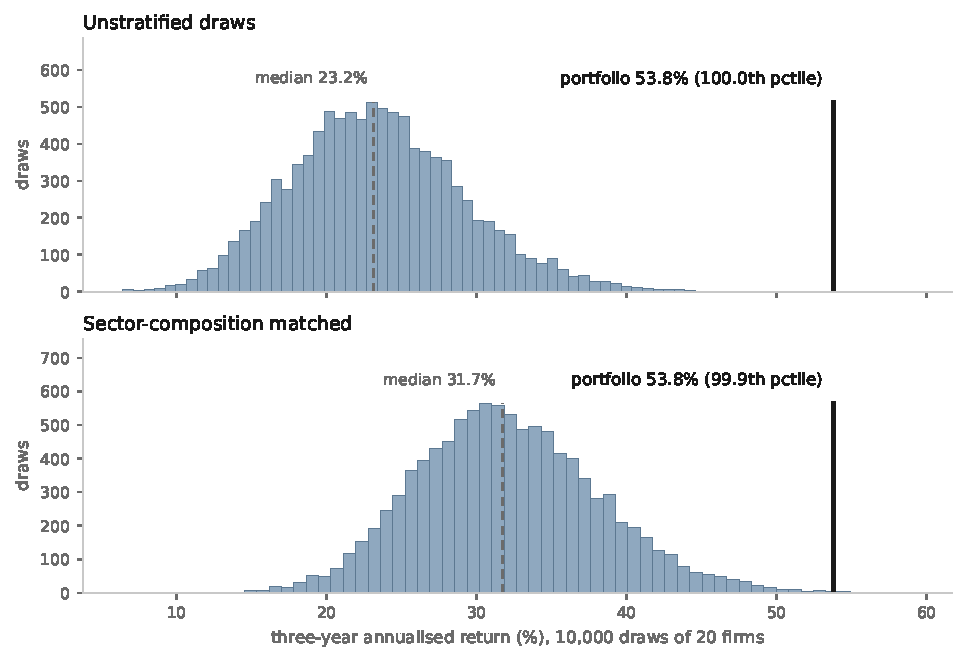
\includegraphics[width=0.92\textwidth]{fig_layer2_v11.pdf}
\caption{\textbf{Layer 2 (randomisation).} \emph{Where the portfolio sits in the placebo
distribution.} Each panel is a separate drawing scheme, so each carries a single series and reads
correctly in greyscale. The dashed rule is the placebo median; the solid rule is the actual
portfolio. Matching sector composition moves the median from \LtwoUnstratMedian\% to
\LtwoMatchedMedian\% --- most of the visible gap in the upper panel is sector allocation. Seed
\LtwoSeed. Percentiles only; no test statistic is computed in this layer.}
\label{fig:layer2}
\end{figure}

% AUTO-GENERATED by scripts/build_wp_tables_v11.py -- do not edit by hand.
\begin{table}[htbp]
\centering\small
\caption{\textbf{Layer 2 (randomisation).} The actual portfolio against 10{,}000 draws of 20 firms from the same 1{,}469-firm 2026 guard-passing pool. Equal weights on both sides. Seed 20260725. Percentiles only: this layer reports no test statistics, because the portfolio embeds 2026 hindsight by construction.}
\label{tab:layer2}
\begin{tabular}{llrrrrrr}
\toprule
Draw scheme & Metric & \multicolumn{5}{c}{Placebo distribution} & Actual \\
\cmidrule(lr){3-7}
& & p5 & p25 & p50 & p75 & p95 & (pctile) \\
\midrule
\multirow{4}{*}{\shortstack[l]{Unstratified\\draws}} & Annualised return & 14.5\% & 19.4\% & 23.2\% & 27.1\% & 33.6\% & \textbf{53.8\%} (100.0) \\
 & Sharpe ratio & 0.78 & 1.03 & 1.22 & 1.41 & 1.70 & \textbf{2.10} (99.9) \\
 & Maximum drawdown & -25.4\% & -23.0\% & -21.5\% & -20.1\% & -18.0\% & \textbf{-30.0\%} (0.0) \\
 & $\beta$ vs.\ TOPIX & 0.67 & 0.73 & 0.77 & 0.81 & 0.87 & \textbf{1.06} (100.0) \\
\midrule
\multirow{4}{*}{\shortstack[l]{Sector-composition\\matched}} & Annualised return & 22.7\% & 27.8\% & 31.7\% & 36.0\% & 42.7\% & \textbf{53.8\%} (99.9) \\
 & Sharpe ratio & 1.11 & 1.34 & 1.51 & 1.68 & 1.94 & \textbf{2.10} (98.8) \\
 & Maximum drawdown & -28.0\% & -25.4\% & -23.8\% & -22.4\% & -20.5\% & \textbf{-30.0\%} (1.6) \\
 & $\beta$ vs.\ TOPIX & 0.80 & 0.85 & 0.89 & 0.93 & 0.99 & \textbf{1.06} (99.7) \\
\bottomrule
\end{tabular}
\begin{minipage}{\textwidth}\vspace{2pt}\scriptsize
\textit{Notes.} Sector matching draws, for each 33-sector code, the same number of firms the actual portfolio holds in that sector. Moving from unstratified to sector-matched draws raises the median placebo return from 23.2\% to 31.7\%, i.e.\ sector composition alone accounts for a large part of the gap to the pool. The portfolio also sits at the extreme of the $\beta$ and drawdown distributions, so its position on the return distribution is not risk-neutral.
\end{minipage}
\end{table}



\subsection{Factor attribution}\label{sec:factors}

We build monthly factors from the same point-in-time filing panel: a market factor (the TOPIX ETF,
with the risk-free rate set to zero, Japanese short rates having been near zero over the sample), a
quality factor sorting on ROE, an accounting-size factor sorting on total assets, a 12-1 month
momentum factor, and an electrical-machinery sector factor. \textbf{There is no value factor.} A
book-to-market sort requires market equity, hence a share count, and for the reason given in
Section~\ref{sec:l1scope} the data does not contain one point-in-time. We report this as a gap
rather than fill it with a proxy that would not mean what its name suggests; the size factor is
likewise labelled an accounting proxy wherever it appears. Table~\ref{tab:factors} reports
\FaMonths\ monthly observations, \FaFirst\ to \FaLast.

Our headline specification is the market factor plus the sector factor, and we fixed that choice on
degrees of freedom before looking at the estimates: \FaMonths\ monthly observations do not support
five regressors. We report the richer models in the same table rather than burying them, and we note
the direction of the choice --- the five-factor alpha is \emph{larger} than the parsimonious one, so
preferring the parsimonious model lowers the alpha we claim.

Three results, in the order that matters for calibration. First, the sector loading is large and
statistically strong (\FaHeadOursSector, $t=\FaHeadOursSectorT$), and the sector factor itself
returned \FaSectorAnn\% annualised --- the semiconductor complex is where this portfolio lived.
Second, the portfolio's alpha does \emph{not} vanish once the sector is controlled for
(\FaHeadOursAlpha\% annualised, $t=\FaHeadOursAlphaT$, adjusted $R^2$ \FaHeadOursRtwo), and this holds
across all four specifications we ran. We could stop there and claim residual selection value. We do
not, because of the third result: \textbf{the mechanical benchmark --- the same quality gate, the same
pool, no discretionary step --- earns a \emph{larger} alpha than the portfolio does}
(\FaHeadBenchAlpha\% versus \FaHeadOursAlpha\% under the headline model, and
\FaBenchAlpha\% versus \FaOursAlpha\% under the five-factor model). Whatever these regressions pick
up, it is not something the discretionary layer added.

A fourth observation ties the layers together. The quality factor that the screen sorts on returned
\FaQmjAnn\% annualised over this sample --- essentially nothing. That is the same message as
Table~\ref{tab:layer1}, arriving through a different route: in this market and this window, sorting on
the accounting quality of Japanese firms did not pay.

\paragraph{What the missing factors would do.} Three limitations of this factor set are worth signing
rather than merely listing, since a reader will otherwise have to guess which way they bite.

\emph{No value factor.} A book-to-market sort needs market equity, hence a share count, and for the
reason given in Section~\ref{sec:l1scope} the data does not contain one point-in-time. We cannot
estimate the omission's effect and do not try. One anchor from data we do have: the deep-value
control built from the same universe returned \FaGrahamAnn\% annualised over the three-year window
against \FaGrahamTopix\% for TOPIX, so value exposure was costly in this regime. If this portfolio
carries the growth tilt its holdings suggest, then omitting a value factor on which it would load
negatively \emph{flatters} the alpha we report rather than depressing it.

\emph{The size factor is an accounting proxy.} SIZE sorts on total assets, not market capitalisation.
A small, high-multiple growth firm has a large market capitalisation but modest assets, so an
accounting sort places it on the ``small'' side more readily than a market-equity sort would. For a
portfolio tilted toward high-multiple names the proxy therefore \emph{understates} true small-cap
exposure, and the size loadings in Table~\ref{tab:factors} should be read as lower bounds on it.

\emph{Thirty-six months is short.} Even the headline model's standard errors rest on three years of
monthly data spanning one regime. Section~\ref{sec:costs} discounts the resulting Sharpe ratio for
the \SpecTotal\ specifications we traversed; nothing discounts it for the shortness of the sample,
and we would not defend any of these alphas as stable.

% AUTO-GENERATED by scripts/build_wp_tables_v11.py -- do not edit by hand.
\begin{table}[htbp]
\centering\small
\caption{\textbf{Attribution (hindsight-formed portfolio).} \emph{Factor attribution, monthly, 36 months.} Factors are built point-in-time from the filing panel: QMJ sorts on ROE, SIZE on total assets (an accounting-size proxy, \emph{not} market capitalisation), MOM on the 12-1 month return, SECTOR is equal-weighted Electric Appliances minus the equal-weighted universe. \textbf{There is no value factor}: a book-to-market sort needs a share count, which this data does not contain point-in-time. Newey--West $t$ (lag 3) in parentheses.}
\label{tab:factors}
\begin{tabular}{lrrrr}
\toprule
& \multicolumn{2}{c}{Portfolio (equal wt.)} & \multicolumn{2}{c}{Mechanical benchmark} \\
\cmidrule(lr){2-3}\cmidrule(lr){4-5}
& \textbf{CAPM${+}$sector} & Five factors & \textbf{CAPM${+}$sector} & Five factors \\
& \scriptsize(headline) & \scriptsize(robustness) & \scriptsize(headline) & \scriptsize(robustness) \\
\midrule
$\alpha$ (annualised) & +12.7\% & +17.8\% & +14.6\% & +23.9\% \\
 & (+2.09) & (+2.29) & (+1.90) & (+3.06) \\
\midrule
MKT & 0.99 & 0.99 & 1.28 & 1.24 \\
 & (+6.76) & (+4.06) & (+6.40) & (+5.11) \\
QMJ & -- & 0.40 & -- & 1.23 \\
 &  & (+0.89) &  & (+2.09) \\
SIZE & -- & 0.66 & -- & 1.09 \\
 &  & (+2.21) &  & (+3.92) \\
MOM & -- & 0.15 & -- & 0.32 \\
 &  & (+0.27) &  & (+1.06) \\
SECTOR & 0.82 & 0.98 & 0.44 & 0.69 \\
 & (+2.82) & (+3.44) & (+1.25) & (+1.79) \\
\midrule
Adjusted $R^2$ & 0.72 & 0.75 & 0.59 & 0.70 \\
\midrule
\multicolumn{5}{l}{\textit{$\alpha$ (annualised) across every specification we ran}} \\
\quad CAPM (1 regressor) & \multicolumn{2}{c}{+12.6\% (+1.54)} & \multicolumn{2}{c}{+14.5\% (+2.04)} \\
\quad CAPM${+}$sector (2 regressors) & \multicolumn{2}{c}{+12.7\% (+2.09)} & \multicolumn{2}{c}{+14.6\% (+1.90)} \\
\quad Four factors (4 regressors) & \multicolumn{2}{c}{+16.0\% (+1.46)} & \multicolumn{2}{c}{+22.6\% (+3.31)} \\
\quad Five factors (5 regressors) & \multicolumn{2}{c}{+17.8\% (+2.29)} & \multicolumn{2}{c}{+23.9\% (+3.06)} \\
\bottomrule
\end{tabular}
\begin{minipage}{\textwidth}\vspace{2pt}\scriptsize
\textit{Notes.} \textbf{The headline specification is CAPM${+}$sector}, chosen on degrees of freedom alone and fixed before the estimates were inspected: 36 monthly observations do not support five regressors. The choice is not self-serving --- the five-factor $\alpha$ is \emph{larger}, so preferring the parsimonious model lowers the $\alpha$ we report. The regressions are run on portfolios formed with 2026 information, so these alphas measure how much in-sample excess return tradable factor exposures span --- not skill. Two features matter for the paper's calibration. The sector loading is large and the portfolio's alpha does \emph{not} vanish once it is included; but the mechanical benchmark, built from the same gate with no discretionary step, earns a \emph{larger} alpha under the headline model (+14.6\% vs.\ +12.7\%) and under every specification in the lower panel. And the quality factor the screen sorts on returned -0.1\% annualised over the sample, consistent with the Layer 1 null. With 36 monthly observations spanning one regime, every alpha here is fragile --- the headline model keeps only two regressors precisely because five is more than this sample supports; see Section~\ref{sec:costs}.
\end{minipage}
\end{table}



\subsection{Implementation and statistical housekeeping}\label{sec:costs}

The contest edition rebalanced to fixed weights daily, which no one can do. Table~\ref{tab:costs}
makes monthly rebalancing with a \CostOneWay\ bp one-way cost plus a \CostOddLot\ bp odd-lot spread
assumption the headline convention and relegates the daily convention to the appendix.

Costs turn out not to matter much here, and we report that as a fact rather than banking it as a
robustness win. Annualised turnover under monthly rebalancing is only \CostTurnover$\times$, because
the portfolio is a buy-and-hold list whose weights drift rather than a signal that trades; the
headline convention returns \CostHeadlineAnn\% against \CostContestAnn\% for the contest convention,
a drag of \CostDrag\ percentage points. Even at \CostGridMax\ bp one-way the series returns
\CostHundredBp\%; Appendix Table~\ref{tab:cost-sens} gives the full grid alongside the contest
edition's daily convention. A reader who suspects our conclusions rest on ignoring frictions can stop
suspecting that; the conclusions rest on the identification problems in
Sections~\ref{sec:power} and~\ref{sec:layer2}, which costs do nothing to fix.

The deflated Sharpe ratio is the one place where we expected our numbers to break and they did not.
Against a trial count of \SpecTotal\ and the fat tails of this series (kurtosis \DsrKurtosis), the
threshold Sharpe is \DsrThreshold\ and the observed arithmetic Sharpe is \DsrObserved, giving a
deflated Sharpe probability of \DsrProb. We draw the modest inference that is actually available:
the portfolio's Sharpe ratio is not an artefact of having tried \SpecTotal\ things. It remains a
Sharpe ratio earned by a portfolio selected with 2026 information, whose mechanical benchmark clears
the same bar, so surviving deflation does not convert it into evidence of selection skill.

\paragraph{Specification count.} The \SpecTotal\ specifications break down as follows, generated from
the same enumeration the deflation uses: \SpecBreakdown. The Layer 1 figure includes a discarded
earnings-yield branch, which we count because we ran it before discovering the share-count coverage
problem, even though its results are not reported. This total is a \emph{lower bound}: informal
variants explored before any artefact was written are not recoverable from the record, and we do not
pretend to have counted them.

% AUTO-GENERATED by scripts/build_wp_tables_v11.py -- do not edit by hand.
\begin{table}[htbp]
\centering\small
\caption{\textbf{Attribution (hindsight-formed portfolio).} \emph{Implementation cost and the deflated Sharpe ratio.} Costs are charged on traded notional (buys plus sells) with an entry cost on the full notional. The deflated Sharpe ratio discounts the observed Sharpe for 85 enumerated specifications and for non-normality \citep{BaileyLopezdePrado2014}.}
\label{tab:costs}
\begin{tabular}{lrrrr}
\toprule
& \multicolumn{2}{c}{Portfolio} & \multicolumn{2}{c}{Mech.\ benchmark} \\
\cmidrule(lr){2-3}\cmidrule(lr){4-5}
Convention & Ann.\ ret. & Sharpe & Ann.\ ret. & Sharpe \\
\midrule
Monthly rebalancing, no cost & 53.6\% & 2.10 & 58.8\% & 2.11 \\
\textbf{Monthly rebalancing, 25 bp + 15 bp odd lot} \emph{(headline)} & 52.8\% & 2.07 & 57.9\% & 2.07 \\
\midrule
Annualised turnover (monthly) & 1.07$\times$ & -- & 1.15$\times$ & -- \\
\midrule
\multicolumn{5}{l}{\textit{Deflated Sharpe ratio on the headline series (arithmetic Sharpe; see note)}} \\
Observed Sharpe (arithmetic) &  & 1.79 &  & 1.78 \\
Threshold Sharpe from 85 trials &  & 0.63 &  & 0.63 \\
Deflated Sharpe probability &  & 0.972 &  & 0.972 \\
\bottomrule
\end{tabular}
\begin{minipage}{\textwidth}\vspace{2pt}\scriptsize
\textit{Notes.} The contest edition's daily fixed-weight convention, which is not implementable, is reported in Appendix Table~\ref{tab:cost-sens} together with the full cost grid. Costs barely matter here, and we report that rather than claiming a robustness win: annualised turnover under monthly rebalancing is only 1.07$\times$, so the headline convention costs the portfolio 1.0 percentage points relative to the contest convention. \textbf{The Sharpe ratio in this table is arithmetic} (mean/sd of daily net returns, annualised), because that is what the deflated Sharpe formula is defined on; it is lower than the geometric Sharpe of 2.07 reported in Tables~\ref{tab:layer2} and~\ref{tab:dof}. The deflated Sharpe survives at the 95\% level --- but so does the mechanical benchmark's, and both series embed 2026 hindsight, so this is a statement about dispersion in the pool, not about skill.
\end{minipage}
\end{table}



\section{Benchmarks are distributions, not points}\label{sec:benchmark}

A comparison in this literature is usually reported as a number: the benchmark returned $x$. Our
second contribution is a measurement of how little that number constrains anything. Fix the pool and
fix the quality gate, so that the set of firms a researcher may hold is identical. Then vary only two
choices that no referee would think to query --- how many of them to hold, and how to weight them.
Table~\ref{tab:dof} reports the \DofVariants\ resulting variants. The three-year annualised return
runs from \DofMin\% to \DofMax\%, a spread of \DofSpread\ percentage points.

The point is not that our portfolio wins against some of these and loses against others, although
it does. It is that a researcher who has already chosen the pool retains enough freedom to place the
benchmark almost anywhere in a range wide enough to contain most conclusions one might wish to draw
--- and that this freedom is invisible in a paper that reports one benchmark number. Our own
experience is the illustration: the ordering disclosure in Section~\ref{sec:limitations} exists
because we made one of these choices, on a defensible principle, \emph{after} seeing what the other
choice implied. A benchmark should be reported as a distribution over defensible construction
choices, with the choice actually made identified within it.

% AUTO-GENERATED by scripts/build_wp_tables_v11.py -- do not edit by hand.
\begin{table}[htbp]
\centering\small
\caption{\textbf{Layer 3 (descriptive): the benchmark is a distribution.} The same pool and the same quality gate, varying only two ordinary construction choices --- how many firms to hold and how to weight them. Three-year annualised returns to 2026-06-01.}
\label{tab:dof}
\begin{tabular}{llrrrr}
\toprule
Holdings & Weighting & Ann.\ return & Sharpe & MDD & $\beta$ \\
\midrule
12 & Start-of-window cap.\ weighted & 29.1\% & 1.13 & -25.8\% & 0.99 \\
12 & End-of-window cap.\ weighted & 42.6\% & 1.35 & -32.7\% & 1.18 \\
12 & Equal weighted & 34.6\% & 1.37 & -27.9\% & 1.01 \\
15 & Start-of-window cap.\ weighted & 33.6\% & 1.28 & -26.3\% & 1.03 \\
15 & End-of-window cap.\ weighted & 80.6\% & 2.24 & -34.0\% & 1.37 \\
15 & Equal weighted & 49.4\% & 1.81 & -27.8\% & 1.13 \\
20 & Start-of-window cap.\ weighted & 40.7\% & 1.37 & -30.8\% & 1.14 \\
20 & End-of-window cap.\ weighted & 74.1\% & 2.05 & -35.6\% & 1.37 \\
20 & Equal weighted & 58.7\% & 2.10 & -29.4\% & 1.16 \\
\midrule
\multicolumn{2}{l}{\textbf{Range across the 9 variants}} & \textbf{29.1\%--80.6\%} & & & \\
\bottomrule
\end{tabular}
\begin{minipage}{\textwidth}\vspace{2pt}\scriptsize
\textit{Notes.} Descriptive statistics only. The spread of 51.5 percentage points is produced entirely by construction choices a researcher makes after the pool is fixed --- not by any difference in the firms available to hold.
\end{minipage}
\end{table}



\section{Limitations}\label{sec:limitations}

\paragraph{The ordering disclosure.} Our main comparison weights the benchmark by
start-of-window capitalisation. We adopted that weighting \emph{after} observing that our portfolio
underperformed the end-of-window weighting, on the principle --- which we still hold --- that a
portfolio weight must not embed information from after the date it is applied. The principle is
correct and the resulting choice is the defensible one. The order in which the two occurred is
nonetheless a fact a reader is entitled to, and no reading of our conduct is available to us that
excludes it. Table~\ref{tab:dof} is the constructive response: we report the whole distribution of
weighting choices rather than asking to be trusted on one.

\paragraph{The fifteen discretionary holdings are not reproducible.} Stated in
Section~\ref{sec:l1scope} and repeated here because it bounds everything: Layer 1 validates the
quality gate and its quality ranking, not the portfolio, and no as-of reconstruction of the
disclosure reading is possible. The Layer 1 deviations compound this --- the translated loss-free
gate, and the ranking that drops the valuation leg for want of point-in-time share counts.

\paragraph{Survivorship, direction stated, magnitude not estimated.} We attempted to retrieve the
JPX delisted-companies list; the request returned HTTP 403 and we did not pursue it further, so
\textbf{the bias is not quantified and we do not estimate it.} What we can state is its direction and
the panel's character. Our price panel covers \SurvTickers\ tickers from \SurvStart\ to
\SurvEnd, and exactly \SurvStopped\ ticker's series stops more than \SurvThreshold\ days before the panel ends:
this is a survivors-only panel. Every historical series in this paper is therefore biased upward ---
our portfolio, the mechanical benchmark, TOPIX as we measure it, and all
\LtwoDraws\ placebo draws alike --- because the universe has had its worst outcomes removed before
we sampled from it. One consequence is mildly favourable to our design and we state it without
leaning on it: since the bias inflates the placebo distribution too, the Layer 2 percentile is less
exposed than a raw return difference would be. That is a reason to prefer the randomisation framing,
not evidence that the bias is small.

\paragraph{The randomisation matches sectors, not risk.} Our placebo draws match the portfolio's size
and, in the stratified variant, its sector composition. They do not match its risk. The portfolio is a
concentrated bet whose beta sits at the \LtwoMatchedBetaPctile th percentile of the matched
distribution against a median of \LtwoMatchedBetaMedian, so part of its return percentile is
compensation for carrying more market exposure than a typical draw. The natural next design is a
beta- or volatility-matched placebo, and \textbf{we did not run one}. We report the beta and drawdown
percentiles alongside the return percentile so that a reader can see the confound rather than take our
word that it is small --- we do not know that it is small.

\paragraph{One market, one regime, and windows that are not a sample.} Everything here is Japanese
equities between \SurvStart\ and \SurvEnd, a period containing an unusually strong advance in exactly
the sector this portfolio concentrates in. Layer 1 has \LoneNasof\ as-of dates whose pools overlap
heavily; that is three overlapping views of one regime, not three observations. Section~\ref{sec:power}
gives the detection thresholds this implies, and they are large.

\paragraph{The evidence ladder is a proposal, not a result.} It is unvalidated as a predictor, its
level-2 and level-3 assignments rest on \LadderVerified\ hand codings with no inter-coder agreement
statistics, and Section~\ref{sec:ladder-validation} states what a validation would require rather
than gesturing at one.

\paragraph{What we would revise first.} If a reader grants us one further analysis, we would spend it
on validating the ladder rather than on extending the return evidence. The return evidence is
constrained by data we cannot obtain --- point-in-time share counts, a delisting list, a longer panel,
more regimes --- whereas the measurement claim in Section~\ref{sec:measurement} is testable now with
the artefacts we already have.

\section{Conclusion}\label{sec:conclusion}

A widely used measure of thematic exposure turns out, in a full cross-section of Japanese listed
firms, to be a sector label: \SatDistinct\ distinct values across \SatFirms\ firms,
\SatSectorShare\% of firms exactly at their sector's median, and a mechanism ---
metadata-only keyword matching, a hard-coded sector bonus, and a quarter of the weight resting on an
input populated for \SatRdPresent\ firms --- that leaves nothing varying within a sector. We proposed a
disclosure-graded evidence ladder as the alternative, defined it as a coding protocol so that its
assignments can be re-opened and disputed, and then found that our own portfolio clears it for
\OwnVerified\ of \OwnHoldings\ holdings.

On the performance question that motivated the project, our answer is negative and bounded. Run
forward from filings actually on file, the mechanical quality screen underperformed in
\LoneNegative\ of \LoneCells\ specification cells, though the design is too weak to distinguish that
from zero at \MdeNotDetectable\ of \MdeTotal\ as-of dates. The full portfolio sits high in a randomisation
distribution --- and equally high in that distribution's beta and drawdown tails. Its factor alpha
survives a sector control, but the purely mechanical benchmark's alpha is larger. Costs do not change
any of it and the Sharpe ratio survives deflation for \SpecTotal\ specifications. Taken together these
say the in-sample record cannot be attributed to the mechanical screen, and that nothing in our design
identifies a contribution from the discretionary layer.

What we would ask a reader to take from the paper is the measurement claim, not the portfolio. The
diagnostic that exposed the saturated measure costs two lines of code --- count the distinct values a
proposed exposure measure takes, and the share of firms sitting at their sector's median --- and we
would not have thought to run it on a measure we were already using had the sort not visibly failed.
The ladder that replaces it remains unvalidated, and designing that validation is the question we
would most value a reader's view on.

\bibliography{referee_wp_v11}
\appendix
\section*{Appendix}
% AUTO-GENERATED by scripts/build_wp_tables_v11.py -- do not edit by hand.
\begin{table}[htbp]
\centering\small
\caption{\textbf{Layer 1 point-in-time funnel and test statistics.} Firm counts use only filings submitted strictly before the as-of date.}
\label{tab:layer1-t}
\begin{tabular}{lrrr}
\toprule
& 2024-10-01 & 2025-04-01 & 2025-10-01 \\
\midrule
Filings on file & 5,932 & 6,866 & 9,508 \\
Firms on file & 3,575 & 3,575 & 3,577 \\
Firms with $\geq 2$ fiscal years & 2,357 & 3,288 & 3,574 \\
Firms screenable & 2,224 & 3,111 & 3,377 \\
Passing the quality gate & 87 & 153 & 176 \\
With a usable price series & 87 & 153 & 176 \\
Measurement start & 2024-09-30 & 2025-03-31 & 2025-09-30 \\
\midrule
\multicolumn{4}{l}{\textit{Newey--West $t$ on daily excess vs.\ TOPIX}} \\
Top 5, ROE rank & -1.10 & -1.92 & -1.28 \\
Top 20, ROE rank & -1.08 & -0.48 & -1.51 \\
Top 5, ROE${+}$margin rank & -1.46 & -0.28 & -0.98 \\
Top 20, ROE${+}$margin rank & -1.12 & -0.41 & -1.49 \\
\emph{Entire gate-passing pool} & -2.36 & -1.94 & -3.15 \\
\bottomrule
\end{tabular}
\end{table}

\begin{table}[htbp]
\centering\small
\caption{\textbf{Layer 3 (descriptive).} \emph{Gate-threshold stability of the mechanical selection.} Each variant perturbs exactly one threshold and re-runs the selection on the 2026 snapshot; there is no forward measurement here. Overlap counts how many of the 5 base holdings survive.}
\label{tab:robustness}
\begin{tabular}{lc}
\toprule
Variant (one threshold changed) & Overlap with base \\
\midrule
ROE threshold $\geq$12\% & 4 of 5 \\
ROE threshold $\geq$18\% & 5 of 5 \\
Operating margin $\geq$5\% & 4 of 5 \\
Equity ratio $\geq$40\% & 4 of 5 \\
Drop the revenue/profit-growth gate & 4 of 5 \\
Drop the loss-free gate & 4 of 5 \\
Rank on ROE alone & 4 of 5 \\
Sector cap raised to 3 & 5 of 5 \\
\midrule
\textbf{Minimum overlap across all 8 variants} & \textbf{4 of 5} \\
\bottomrule
\end{tabular}
\begin{minipage}{\textwidth}\vspace{2pt}\scriptsize
\textit{Notes.} Stability here is a property of the \emph{selection rule} on one snapshot, not evidence about returns. The mechanical selection is stable to single-threshold perturbation: at least 4 of 5 holdings survive every variant. This says the \emph{selection} is not knife-edge; it says nothing about whether the selection has forward-looking content, which Table~\ref{tab:layer1} addresses and answers in the negative.
\end{minipage}
\end{table}

\begin{table}[htbp]
\centering\small
\caption{\textbf{Attribution (hindsight-formed portfolio).} \emph{Cost sensitivity and the contest edition's daily convention.} Three-year annualised returns. The odd-lot spread of 15 bp is added to every one-way cost in the grid.}
\label{tab:cost-sens}
\begin{tabular}{lrrrrrrrr}
\toprule
& \multicolumn{5}{c}{Monthly rebalancing, one-way cost} & \multicolumn{2}{c}{Daily rebalancing} & Turnover \\
\cmidrule(lr){2-6}\cmidrule(lr){7-8}
Series & 0 bp & 10 bp & 25 bp & 50 bp & 100 bp & no cost & headline & (monthly) \\
\midrule
Portfolio (equal weight) & 53.3\% & 53.1\% & 52.8\% & 52.2\% & 51.2\% & 53.8\% & 50.9\% & 1.07$\times$ \\
Mechanical benchmark & 58.4\% & 58.2\% & 57.9\% & 57.3\% & 56.1\% & 58.7\% & 55.6\% & 1.15$\times$ \\
\bottomrule
\end{tabular}
\begin{minipage}{\textwidth}\vspace{2pt}\scriptsize
\textit{Notes.} The daily fixed-weight convention is the contest edition's and is not implementable; it appears here rather than in the main text. Even a 100 bp one-way assumption leaves the ranking of the two series unchanged, which is why Section~\ref{sec:costs} declines to treat cost robustness as a result.
\end{minipage}
\end{table}

\begin{table}[htbp]
\centering\small
\caption{\textbf{Measurement audit (no inference layer).} \emph{Evidence level against realised revenue growth --- the result runs against our own proposal.} The 14 hand-coded firms; annualised total revenue growth across the fiscal years on file.}
\label{tab:correspondence}
\begin{tabular}{lrrrr}
\toprule
Evidence level & $n$ & Median & Mean & Range \\
\midrule
Level 2 & 8 & +13.5\% & +14.5\% & -1.1\% to +28.3\% \\
Level 3 & 6 & +7.8\% & +7.5\% & -2.2\% to +21.3\% \\
\bottomrule
\end{tabular}
\begin{minipage}{\textwidth}\vspace{2pt}\scriptsize
\textit{Notes.} \textbf{Level-3 firms grew revenue more slowly than level-2 firms over this window.} We report this rather than omit it. It is not evidence that the ladder fails and we would resist a reader concluding either way: the cells hold 8 and 6 firms, the measure is \emph{total} revenue rather than theme-attributable revenue (which almost no firm discloses separately), the levels were not coded as-of, and nothing controls for sector or size. The table has no power to order the levels --- which is precisely the point made in Section~\ref{sec:ladder-validation}.
\end{minipage}
\end{table}



\subsection*{Replication}

Every number above is produced by a script and written to a JSON file that the manuscript reads
through a generator; no number is typed into the \LaTeX\ source, and a machine check fails the build
if one is. The scripts, the JSON outputs, and a README giving the command for each table are in
\texttt{referee\_package\_v11/}. The random seed is \LtwoSeed\ and appears both in
\texttt{build\_layer2\_placebo\_v11.py} and in Section~\ref{sec:layer2}.

Run order, because later scripts read earlier outputs:

\begin{enumerate}\itemsep0pt\parskip0pt
\item \texttt{build\_layer1\_pit\_v11.py}
\item \texttt{build\_layer2\_placebo\_v11.py}
\item \texttt{build\_factors\_v11.py}
\item \texttt{build\_costs\_v11.py}
\item \texttt{build\_saturation\_v11.py}
\item \texttt{build\_survivorship\_v11.py}
\item \texttt{build\_appendix\_v11.py}
\item \texttt{build\_fig\_layer2\_v11.py}
\item \texttt{build\_wp\_tables\_v11.py}
\item \texttt{check\_gates\_v11.py}
\end{enumerate}

We do not redistribute the price panel, which is vendor data; the README states its schema and
coverage so it can be substituted. The two derived filing tables are described there as well. The
README also lists, in one place, the five deviations forced on us by data we could not obtain --- no
point-in-time share counts, hence no valuation leg in Layer 1 and no value factor; the translated
loss-free gate; the unquantified survivorship direction; and the two distinct Sharpe definitions
that appear in different tables.

\end{document}
